\section{Tau fake scale factor calibration in the ttCRs}
\label{sec:tauFF_appendix}

Figure~\ref{fig:ttCR_mtt} shows the post-fit of the leading $\thad$ $\pt$ in the ttCRs, which shows a good agreement between the data and the fitted background model.
Table~\ref{tab:ff1_summary} and~\ref{tab:ff2_summary} are summarized the fake scale factors of 1-prong and 3-prong taus
derived from the ttCRs including both statistical and systematic uncertainties. 

\begin{figure}[H]
\centering
\begin{tabular}{@{}ccc@{}}
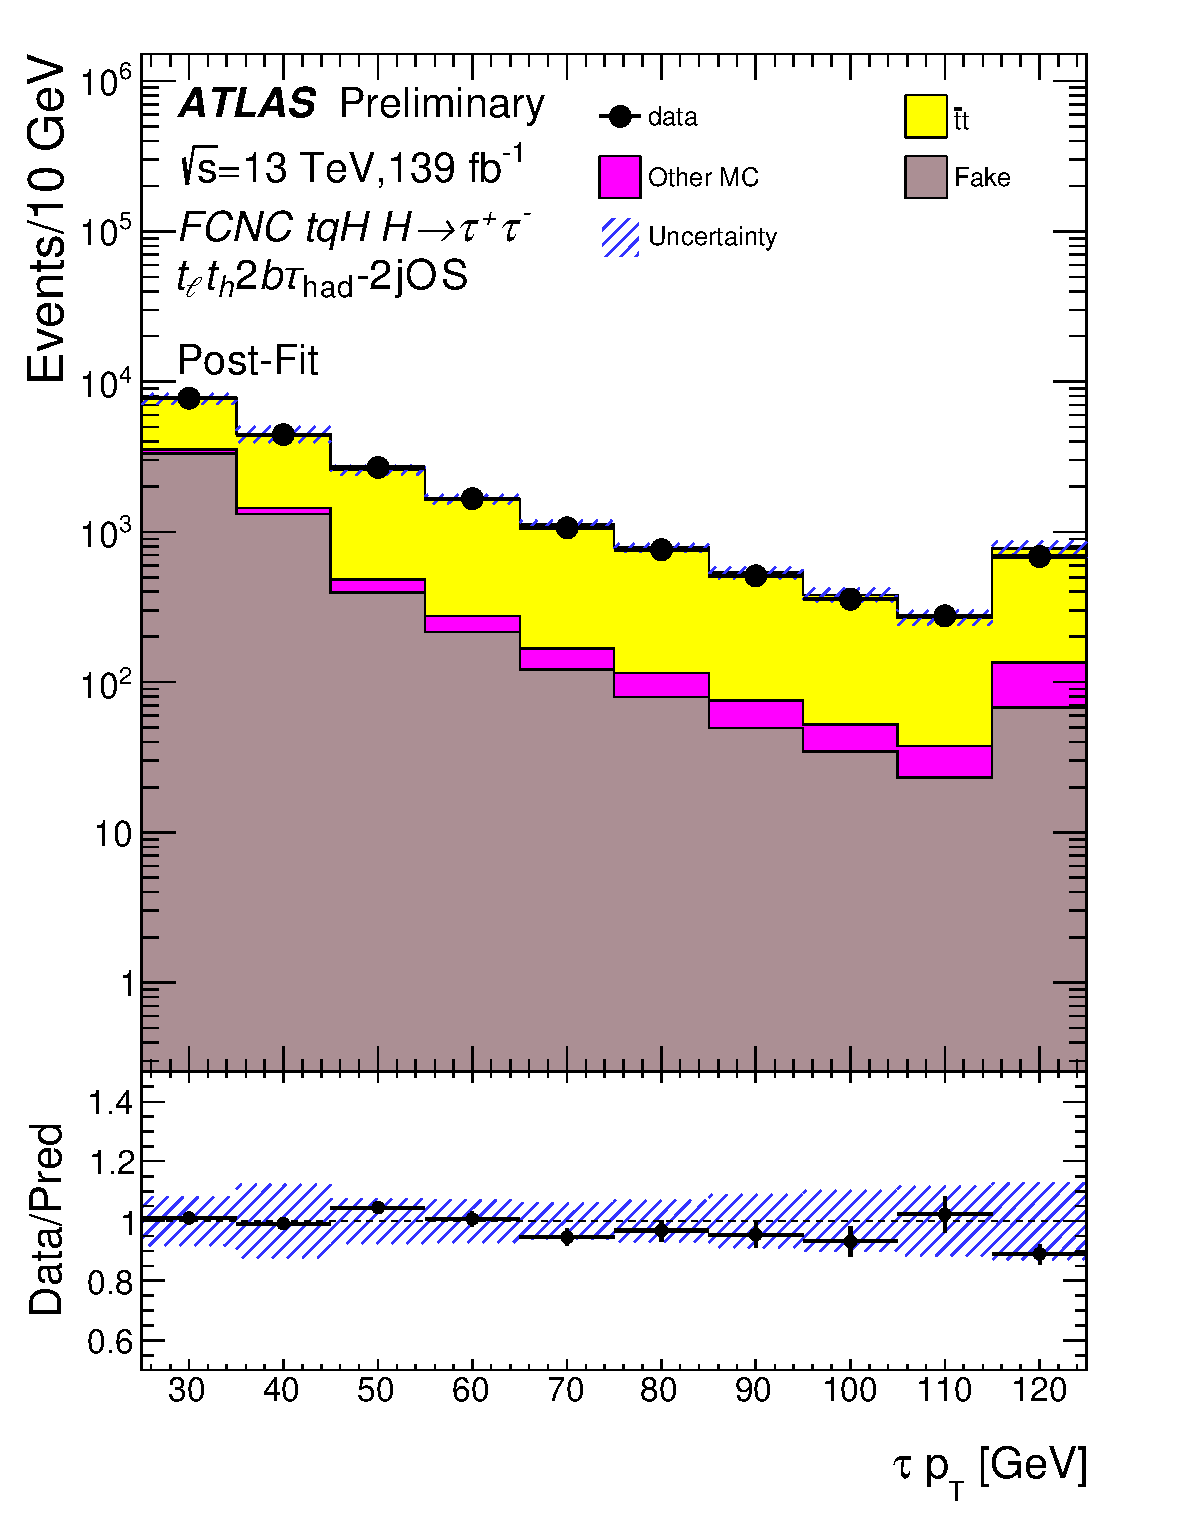
\includegraphics[page=1,width=0.29\textwidth]{figures/ttCR/tuH_reg1l1tau2b2j_os_log_ttCR.pdf} &
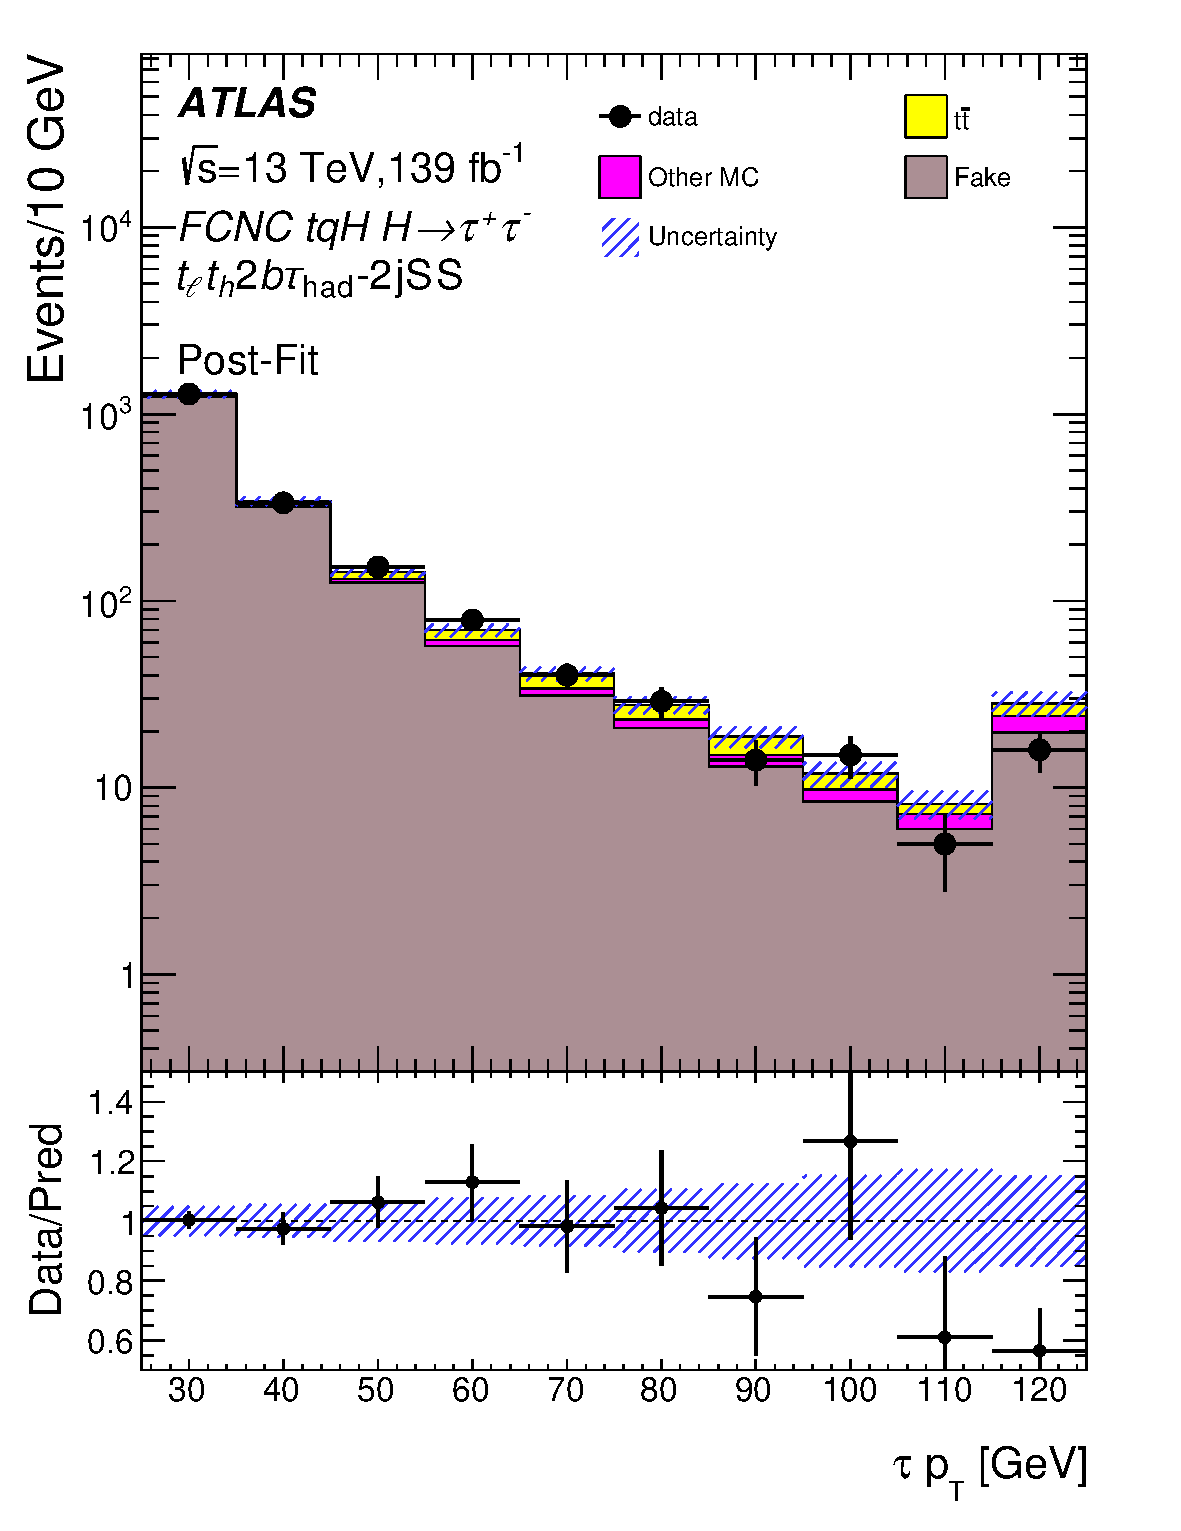
\includegraphics[page=1,width=0.29\textwidth]{figures/ttCR/tuH_reg1l1tau2b2j_ss_log_ttCR.pdf}&
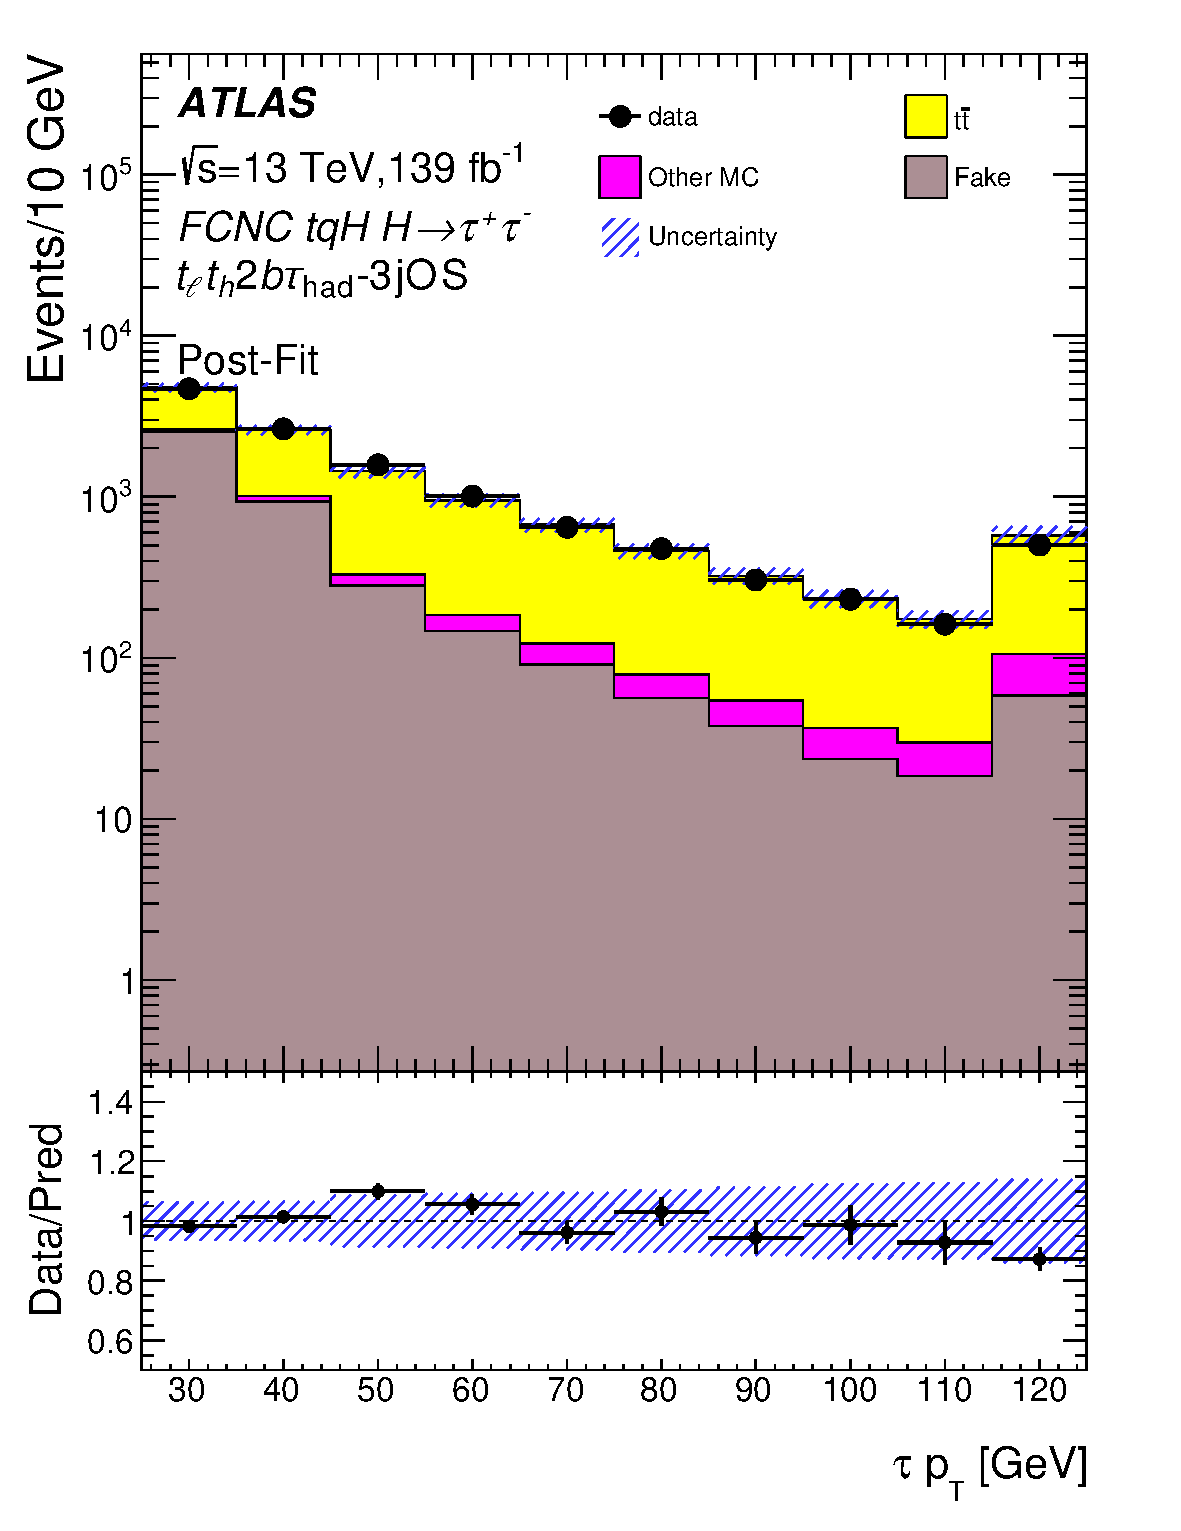
\includegraphics[page=1,width=0.29\textwidth]{figures/ttCR/tuH_reg1l1tau2b3j_os_log_ttCR.pdf}\\
(a) & (b) & (c) \\
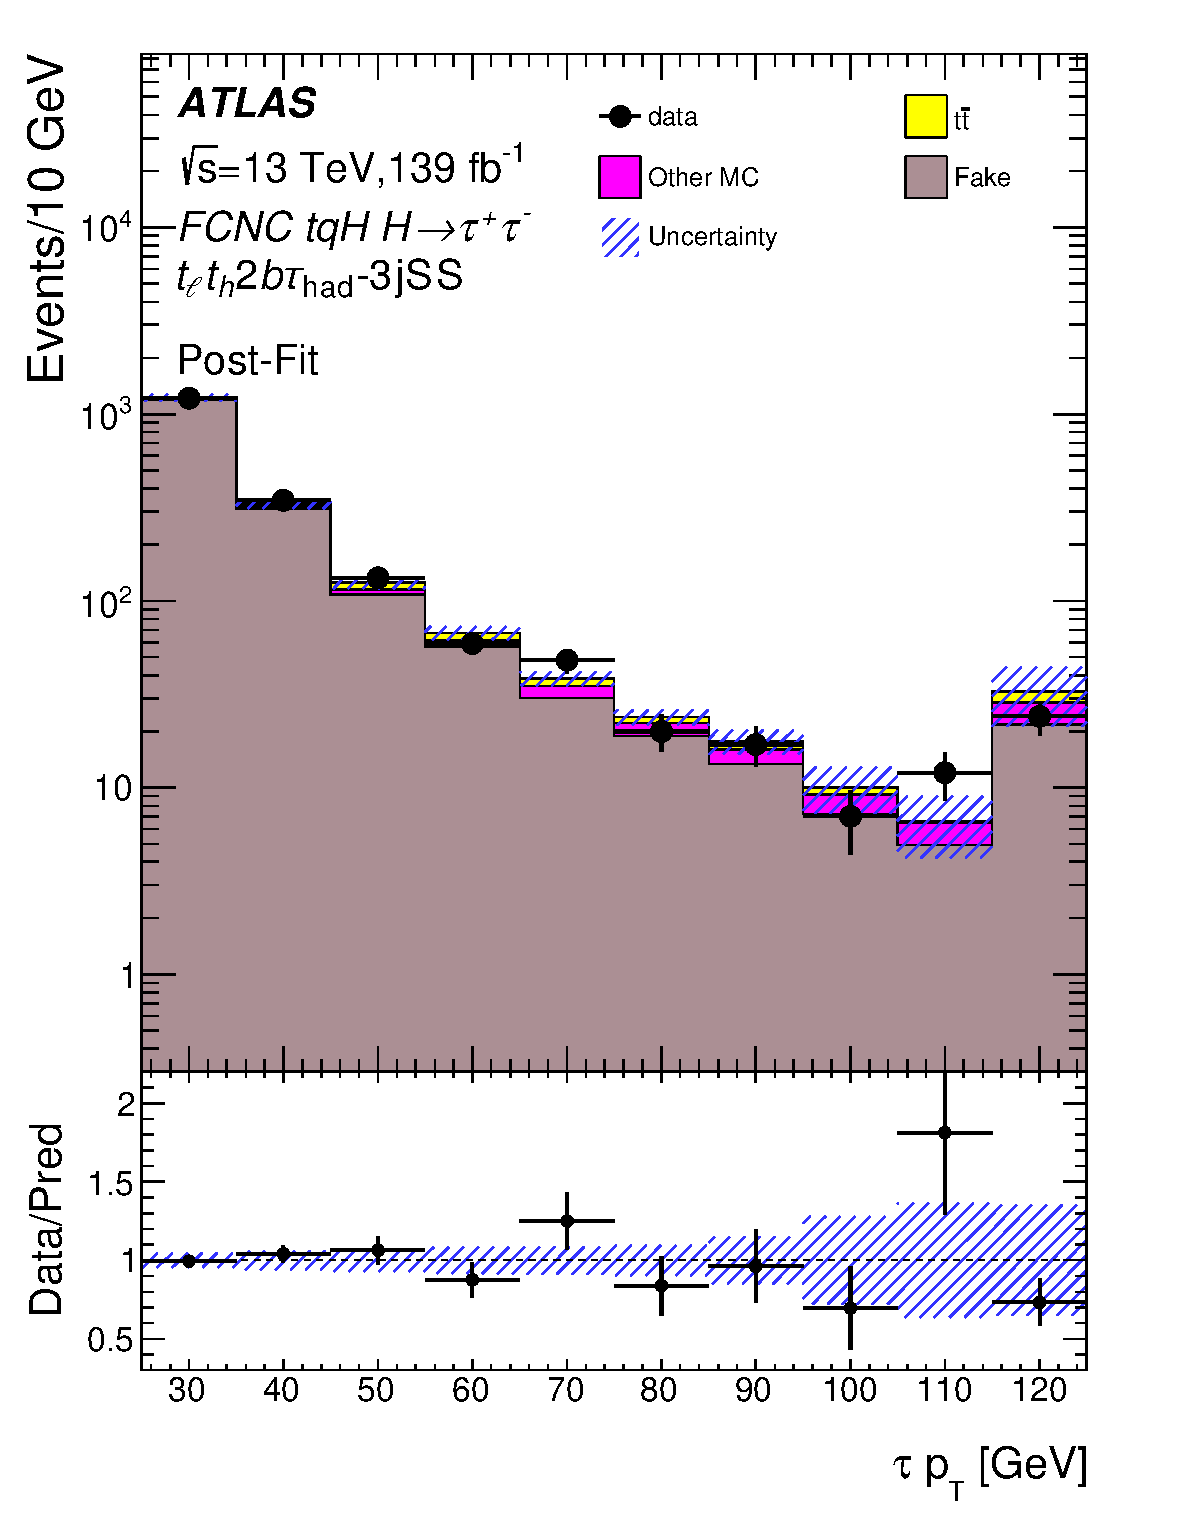
\includegraphics[page=1,width=0.29\textwidth]{figures/ttCR/tuH_reg1l1tau2b3j_ss_log_ttCR.pdf}&
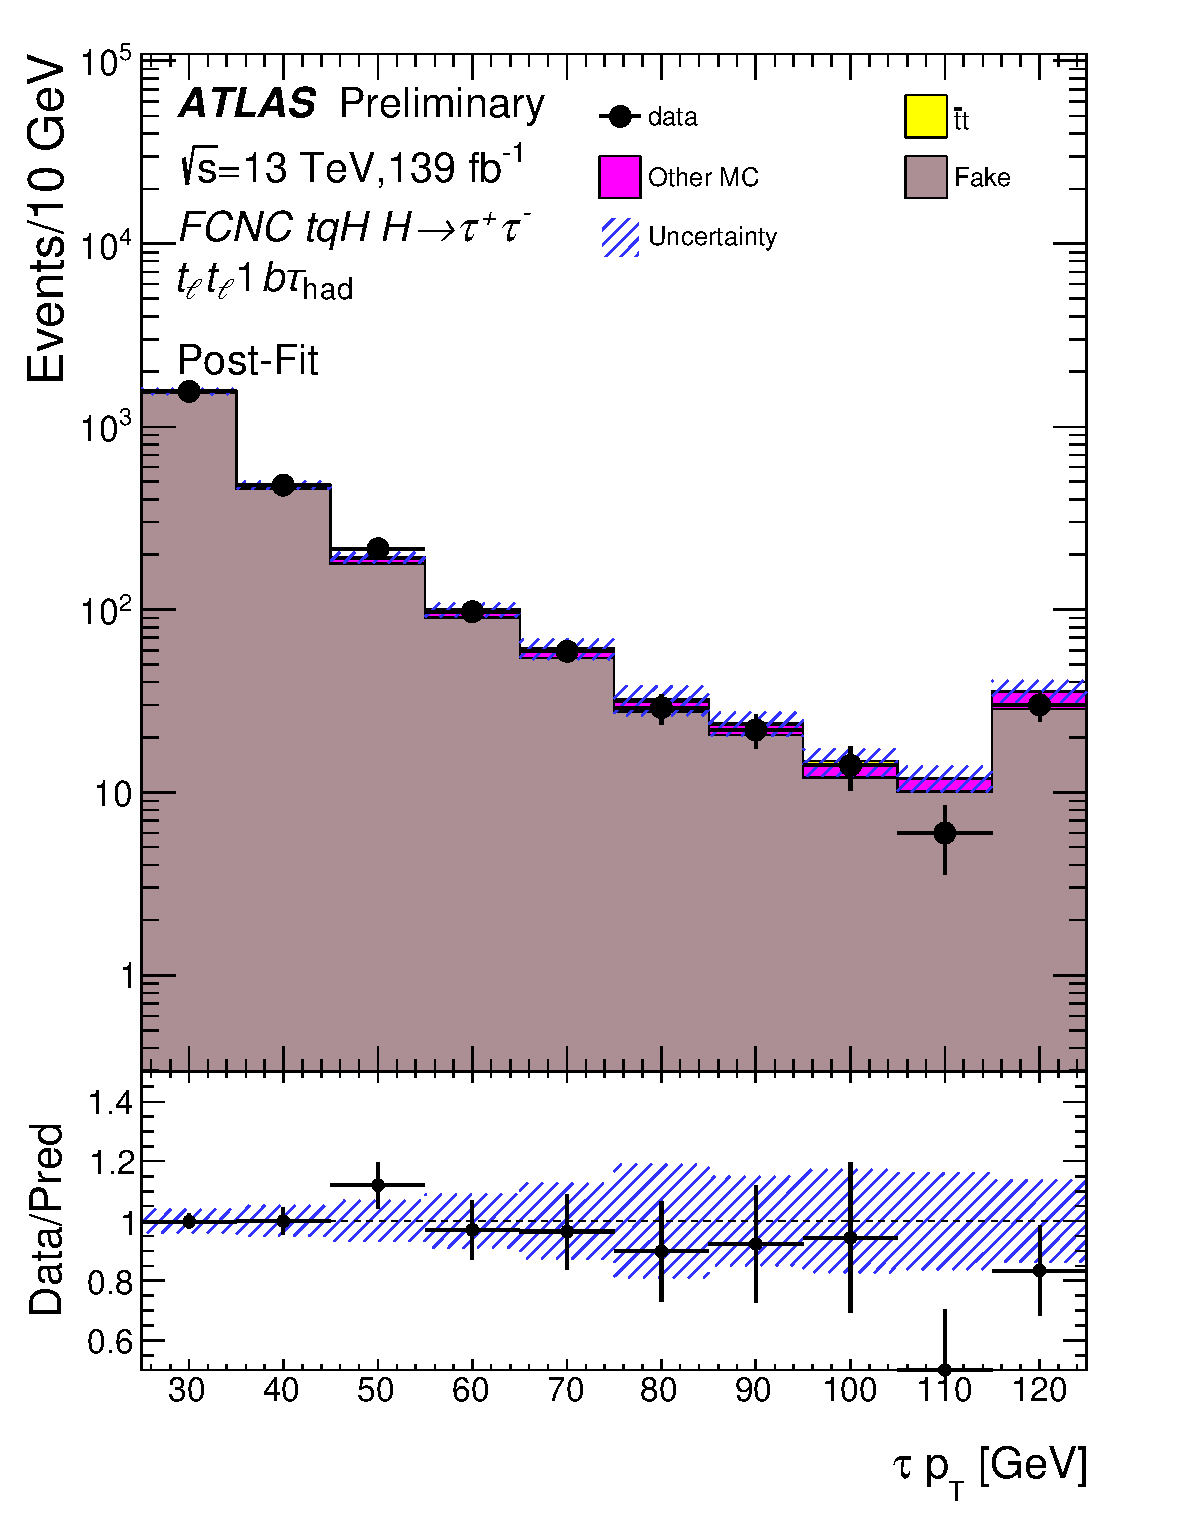
\includegraphics[page=1,width=0.29\textwidth]{figures/ttCR/tuH_reg2l1tau1bnj_log_ttCR.pdf}&
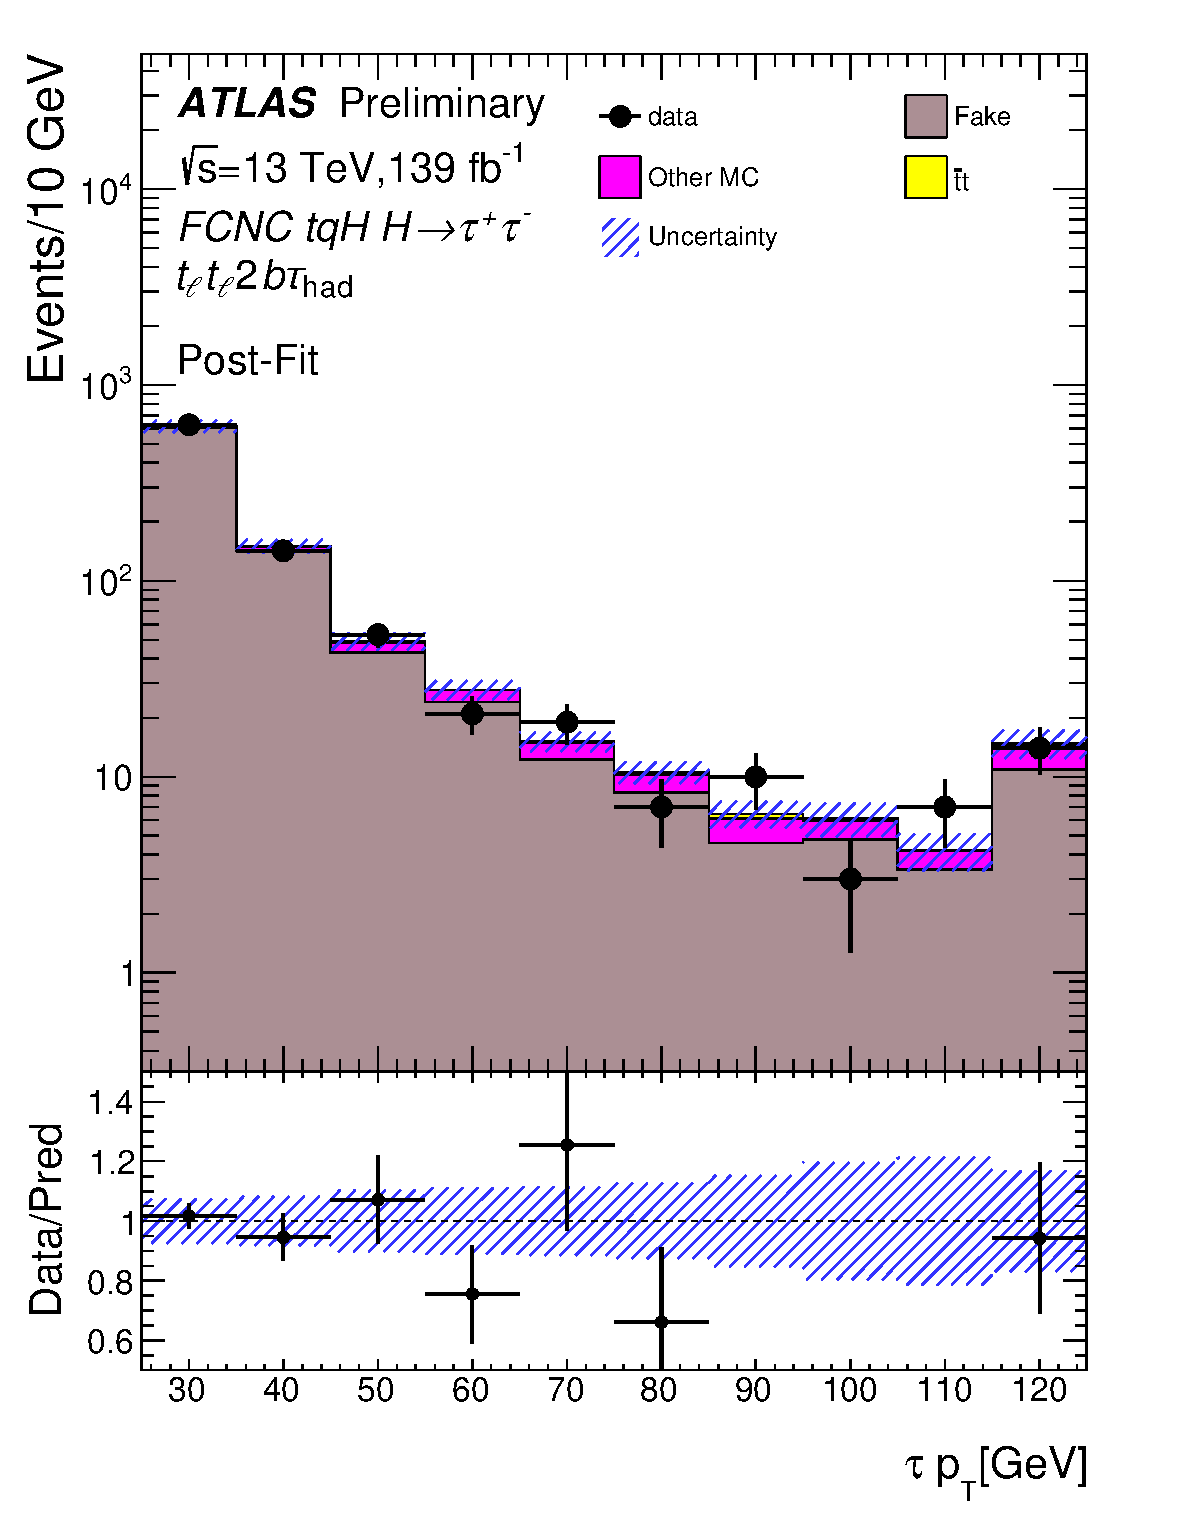
\includegraphics[page=1,width=0.29\textwidth]{figures/ttCR/tuH_reg2l1tau2bnj_log_ttCR.pdf}\\
(d) & (e) & (f)\\
\end{tabular}
\caption{Leading $\thad$ $\pt$  distributions obtained after the fit to data (``Post-Fit'') for the $\thad$ fake scale factors in the following ttCRs:
  $t_{\ell}t_{h}$2b$\thad$-2j OS (a), $t_{\ell}t_{h}$2b$\thad$-2j SS (b), $t_{\ell}t_{h}$2b$\thad$-3j OS (c), $t_{\ell}t_{h}$2b$\thad$-3j SS (d),
  $t_{\ell}t_{\ell}$1b$\thad$-nj (e) and $t_{\ell}t_{\ell}$2b$\thad$-nj (f).
  The total size of the statistical and systematic uncertainties of the background prediction is indicated by the hatched band.
  Overflow events are included in the last bin. The lower panels show the data to prediction ratio.}
\label{fig:ttCR_mtt}
\end{figure}

\begin{table}
\caption{ Summary of fake tau (1-prong) scale factors derived in the ttCRs. The numbers are shown as: nominal values, statistical, and systematics erros. }
\begin{center}
\begin{tabular}{lcccccc}
\toprule\toprule

Fake tau types & \multicolumn{3}{c}{1-prong tau}  \\ \midrule
$\thad$ $\pt$                                   &  $25-35$ GeV  & $35-45$ GeV  &  $45-$ GeV            \\
\midrule
Type-1                          &$0.71 \pm 0.01 \pm 0.03 $ &$0.61 \pm 0.02 \pm 0.04 $ &$0.38 \pm 0.02 \pm 0.05 $  \\
% W fake OS
Type-2                          &$0.76 \pm 0.06 \pm 0.04 $ & $0.37 \pm 0.08 \pm 0.02$ & $0.74 \pm 0.08 \pm 0.02 $ \\
% W fake SS
Type-3                          &$0.62 \pm 0.10 \pm 0.03 $ &$0.83 \pm 0.09 \pm 0.03 $ &$0.94 \pm 0.07 \pm 0.02 $  \\
%  b fake
Type-4                          &$1.20 \pm 0.02 \pm 0.01 $ & $1.01 \pm 0.04 \pm 0.02 $ &$0.76 \pm 0.03 \pm 0.03 $  \\
% other fake
\bottomrule\bottomrule
\end{tabular}
\label{tab:ff1_summary}
\end{center}
\end{table}


\begin{table}
\caption{ Summary of fake tau (3-prong) scale factors derived in the ttCRs. The numbers are shown as: nominal values, statistical, and systematics erros. }
\begin{center}
\begin{tabular}{lcccccc}
\toprule\toprule

Fake tau types        & \multicolumn{3}{c}{3-prong tau}  \\ \midrule
$\thad$ $\pt$                             &  $25-35$ GeV  & $35-45$ GeV       &  $45-$ GeV  \\
\midrule
Type-1                                    & $1.01 \pm 0.03 \pm 0.04 $ & $1.09 \pm 0.04 \pm 0.05 $ & $0.30 \pm 0.05 \pm 0.07 $ \\
% W fake OS
Type-2                                    & $0.93 \pm 0.10 \pm 0.04 $ & $1.05 \pm 0.09 \pm 0.03 $ & $0.79 \pm 0.09 \pm 0.04 $ \\
% W fake SS
Type-3                                    & $1.07 \pm 0.13 \pm 0.03 $ &$1.39 \pm 0.12 \pm 0.03 $ &$1.26 \pm 0.10 \pm 0.04 $  \\
%  b fake
Type-4                                    &$1.28 \pm 0.07 \pm 0.02 $ &$0.66 \pm 0.08 \pm 0.01 $ & $0.71 \pm 0.07 \pm 0.02 $ \\
% other fake
\bottomrule\bottomrule
\end{tabular}
\label{tab:ff2_summary}
\end{center}
\end{table}


